%% Phan cua Thanh vien 1
\subsection{Kích thước công thức}\label{sec:exp-size}

Bảng~\ref{tab:size-cls}, Bảng~\ref{tab:size-vars} và Hình~\ref{fig:size} cho kích thước công thức trên một số đề GEOM. Các số này tính theo Mệnh đề~\ref{prop:size} và đã được đếm lại trực tiếp từ encoder (Mục~\ref{sec:validation}).

\begin{table}[width=\linewidth,pos=t]
\caption{Số mệnh đề (chưa tính $\Delta_K$). Năm cột cuối là các cấu hình \texttt{direct} với AMO tương ứng. Giá trị nhỏ nhất trên mỗi hàng được in đậm.}
\label{tab:size-cls}
\centering\footnotesize
\begin{tabular}{lrrrrrrrrrr}
\toprule
Đề & $n$ & $|E|$ & $H$ & full & pair & Pairwise & Sequential & Binary & Commander & Product \\
\midrule
GEOM20 & 20 & 20 & 25 & \textbf{2\,920} & 6\,320 & 10\,420 & 5\,840 & 6\,920 & 6\,280 & 5\,820 \\
GEOM40 & 40 & 78 & 34 & \textbf{10\,584} & 28\,492 & 45\,692 & 27\,172 & 31\,412 & 29\,012 & 27\,172 \\
GEOM60 & 60 & 185 & 37 & \textbf{22\,330} & 68\,437 & 99\,817 & 66\,277 & 73\,177 & 69\,637 & 66\,457 \\
GEOM80 & 80 & 349 & 52 & \textbf{52\,616} & 180\,466 & 270\,306 & 176\,386 & 189\,186 & 186\,066 & 176\,466 \\
GEOM100 & 100 & 547 & 68 & \textbf{101\,192} & 367\,766 & 568\,866 & 361\,066 & 388\,666 & 382\,166 & 361\,066 \\
GEOM120 & 120 & 773 & 74 & \textbf{149\,444} & 557\,984 & 847\,184 & 549\,224 & 585\,224 & 579\,704 & 549\,464 \\
GEOM60a & 60 & 339 & 60 & \textbf{54\,840} & 205\,520 & 297\,620 & 201\,980 & 213\,020 & 211\,220 & 201\,980 \\
GEOM120a & 120 & 1434 & 110 & \textbf{367\,800} & 1\,551\,542 & 2\,218\,742 & 1\,538\,462 & 1\,591\,742 & 1\,609\,982 & 1\,537\,742 \\
GEOM60b & 60 & 366 & 64 & \textbf{61\,968} & 221\,066 & 326\,966 & 217\,286 & 229\,046 & 228\,746 & 217\,046 \\
GEOM120b & 120 & 1491 & 113 & \textbf{390\,726} & 1\,615\,809 & 2\,321\,529 & 1\,602\,369 & 1\,657\,089 & 1\,678\,089 & 1\,602\,489 \\
\bottomrule
\end{tabular}

\end{table}

\begin{table}[width=\linewidth,pos=t]
\caption{Số biến (chưa tính $\Delta_K$). Năm cột cuối là các cấu hình \texttt{direct} với AMO tương ứng. Giá trị nhỏ nhất trên mỗi hàng được in đậm.}
\label{tab:size-vars}
\centering\footnotesize
\begin{tabular}{lrrrrrrrrrrr}
\toprule
Đề & $n$ & $|E|$ & $H$ & full & compact & pair & Pairwise & Sequential & Binary & Commander & Product \\
\midrule
GEOM20 & 20 & 20 & 21 & 820 & \textbf{400} & 820 & 420 & 820 & 520 & 560 & 620 \\
GEOM40 & 40 & 78 & 28 & 2\,200 & \textbf{1\,080} & 2\,200 & 1\,120 & 2\,200 & 1\,320 & 1\,520 & 1\,560 \\
GEOM60 & 60 & 185 & 33 & 3\,900 & \textbf{1\,920} & 3\,900 & 1\,980 & 3\,900 & 2\,340 & 2\,640 & 2\,700 \\
GEOM80 & 80 & 349 & 42 & 6\,640 & \textbf{3\,280} & 6\,640 & 3\,360 & 6\,640 & 3\,840 & 4\,480 & 4\,400 \\
GEOM100 & 100 & 547 & 52 & 10\,300 & \textbf{5\,100} & 10\,300 & 5\,200 & 10\,300 & 5\,800 & 7\,000 & 6\,700 \\
GEOM120 & 120 & 773 & 61 & 14\,520 & \textbf{7\,200} & 14\,520 & 7\,320 & 14\,520 & 8\,040 & 9\,840 & 9\,240 \\
GEOM60a & 60 & 339 & 52 & 6\,180 & \textbf{3\,060} & 6\,180 & 3\,120 & 6\,180 & 3\,480 & 4\,200 & 4\,020 \\
GEOM120a & 120 & 1434 & 93 & 22\,200 & \textbf{11\,040} & 22\,200 & 11\,160 & 22\,200 & 12\,000 & 14\,880 & 13\,560 \\
GEOM60b & 60 & 366 & 49 & 5\,820 & \textbf{2\,880} & 5\,820 & 2\,940 & 5\,820 & 3\,300 & 3\,960 & 3\,780 \\
GEOM120b & 120 & 1491 & 96 & 22\,920 & \textbf{11\,400} & 22\,920 & 11\,520 & 22\,920 & 12\,360 & 15\,360 & 13\,920 \\
\bottomrule
\end{tabular}

\end{table}

\begin{figure}[pos=t]
\centering
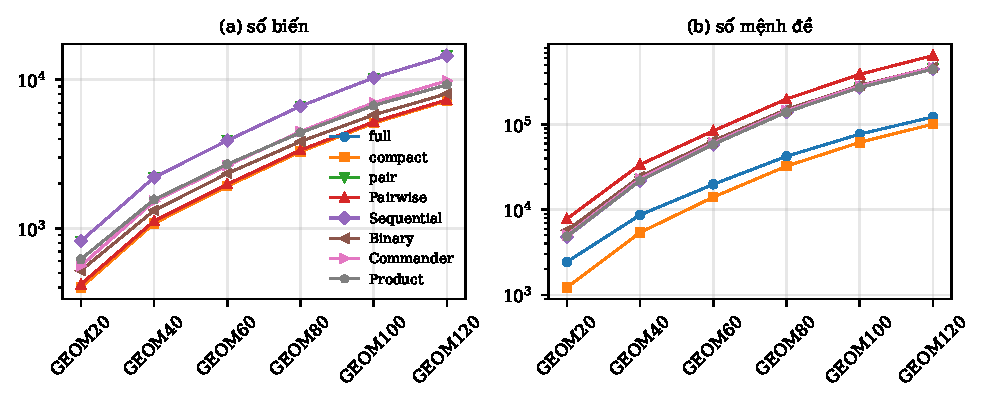
\includegraphics[width=0.92\linewidth]{figures/encoding_size.pdf}
\caption{Kích thước công thức trên họ đề GEOM thưa (thang log).}
\label{fig:size}
\end{figure}

Từ bảng và hình có thể thấy mấy điểm sau (số liệu với $H$ từ heuristic ở Mục~\ref{sec:vars}; trên GEOM120b, $H=96$). Thứ nhất, \texttt{compact} có ít mệnh đề nhất trên mọi đề trong bảng: 297.552 mệnh đề trên GEOM120b, ít hơn \texttt{full} (331.872) vì không có \eqref{eq:channel}. Cả hai đều nhờ mã hóa khoảng: \texttt{full} chỉ bằng 24\% số mệnh đề của \texttt{pair} (1.366.062) dù hai cấu hình có cùng số biến. Thứ hai, \texttt{compact} cũng có ít biến nhất (11.400 so với 22.920 của \texttt{full}); cấu hình \texttt{direct} với pairwise có số biến gần như vậy (11.520) nhưng nhiều mệnh đề nhất (1.867.782). Thứ ba, khác với các bài toán mà AMO chiếm gần hết công thức, ở đây mệnh đề khoảng cách \eqref{eq:pair} áp đảo: trên GEOM120b, 1.320.462 trong 1.354.662 mệnh đề của \texttt{direct} với sequential counter (97,5\%) là mệnh đề khoảng cách. Vì vậy ngoài pairwise, bốn cách mã hóa AMO còn lại có số mệnh đề chỉ chênh nhau khoảng 4\% trên đề này. Tuy vậy, thời gian chạy của solver không chỉ phụ thuộc vào kích thước, nên các con số này chỉ là điểm xuất phát cho các thí nghiệm bên dưới.

\subsection{Kiểm tra tính đúng}\label{sec:validation}

Trước khi đo thời gian, ta kiểm tra encoder bằng các bài kiểm tra trong Bảng~\ref{tab:validation}. Các bài kiểm tra dùng một bộ giải DPLL nhỏ viết kèm trong code, độc lập với các solver CDCL ở Bảng~\ref{tab:solvers}. Tất cả đều đạt.

\begin{table}[width=\linewidth,pos=t]
\caption{Các bài kiểm tra (tất cả đều đạt). Bốn dòng đầu tính cho mỗi cách mã hóa AMO.}
\label{tab:validation}
\centering\small
\begin{tabular}{p{0.74\linewidth}r}
\toprule
Bài kiểm tra & Số trường hợp\\
\midrule
AMO, vét cạn: mọi $2^m$ cách gán cho $x_1,\dots,x_m$ với $m=1,\dots,10$; SAT khi và chỉ khi có nhiều nhất một biến đúng & 2.046\\
AMO, mọi cách gán có 0, 1 hoặc 2 biến đúng, $m=11,\dots,24$ & 2.394\\
Tính lan truyền: UP từ $x_i=1$ suy ra mọi $\neg x_j$, không xung đột, $m=2,\dots,64$, mọi $i$ & 2.079\\
Công thức kích thước AMO (Bảng~\ref{tab:amo}) so với chương trình, $m=2,\dots,200$ & 199\\
\midrule
Tìm kiếm giảm dần so với vét cạn: 200 đồ thị ngẫu nhiên ($n\le 6$, $d\le 4$) $\times$ 10 cấu hình $\times$ 3 chế độ (cận mới; cận cũ first-fit/$d_{\max}+1$ để luôn có lần gọi SAT; cận cũ không loại đỉnh bậc thấp); trạng thái OPT và span trùng với vét cạn & 6.000\\
$F(K)$ thỏa mãn được khi và chỉ khi $\chi_B(G)\le K$, ở mọi $K$, 4 cấu hình & 2.092\\
Công thức kích thước (Mệnh đề~\ref{prop:size}) so với chương trình, 10 cấu hình & 1.000\\
Ví dụ ở Hình~\ref{fig:example}: span 6 ở cả 10 cấu hình, UNSAT tại $K=5$ & 10\\
Trọng số đơn vị trùng với tô màu đồ thị: $K_4$ cần 4 màu, $C_5$ cần 3 màu & 2\\
Số đỉnh và số cạnh đọc từ file trùng với số liệu của~\citet{nguyen2026bcp}, và $LB$ không vượt giá trị tham khảo & 53\\
\bottomrule
\end{tabular}
\end{table}

\subsection{Ảnh hưởng của cách mã hóa}\label{sec:exp-cfg}

Bảng~\ref{tab:res-cfg} so sánh các cấu hình mã hóa khi dùng cùng một solver (\FixedSolver). \AutoCfg

\begin{table}[width=\linewidth,pos=t]
\caption{Ảnh hưởng của cách mã hóa với \FixedSolver: số đề chứng nhận tối ưu / tổng số đề (PAR-2, giây). Ô in đậm là tốt nhất trên mỗi cột.}
\label{tab:res-cfg}
\centering\small
\begin{tabular}{lcccc}
\toprule
Cấu hình & GEOM-S & GEOM-M & GEOM-L & MS-CAP \\
\midrule
\texttt{full} & \textcolor{red}{\textbf{--}} & \textcolor{red}{\textbf{--}} & \textcolor{red}{\textbf{--}} & \textcolor{red}{\textbf{--}} \\
\texttt{no-sym} & \textcolor{red}{\textbf{--}} & \textcolor{red}{\textbf{--}} & \textcolor{red}{\textbf{--}} & \textcolor{red}{\textbf{--}} \\
\texttt{pair} & \textcolor{red}{\textbf{--}} & \textcolor{red}{\textbf{--}} & \textcolor{red}{\textbf{--}} & \textcolor{red}{\textbf{--}} \\
\texttt{non-inc} & \textcolor{red}{\textbf{--}} & \textcolor{red}{\textbf{--}} & \textcolor{red}{\textbf{--}} & \textcolor{red}{\textbf{--}} \\
\midrule
\texttt{direct-pairwise} & \textcolor{red}{\textbf{--}} & \textcolor{red}{\textbf{--}} & \textcolor{red}{\textbf{--}} & \textcolor{red}{\textbf{--}} \\
\texttt{direct-seq} & \textcolor{red}{\textbf{--}} & \textcolor{red}{\textbf{--}} & \textcolor{red}{\textbf{--}} & \textcolor{red}{\textbf{--}} \\
\texttt{direct-binary} & \textcolor{red}{\textbf{--}} & \textcolor{red}{\textbf{--}} & \textcolor{red}{\textbf{--}} & \textcolor{red}{\textbf{--}} \\
\texttt{direct-commander} & \textcolor{red}{\textbf{--}} & \textcolor{red}{\textbf{--}} & \textcolor{red}{\textbf{--}} & \textcolor{red}{\textbf{--}} \\
\texttt{direct-product} & \textcolor{red}{\textbf{--}} & \textcolor{red}{\textbf{--}} & \textcolor{red}{\textbf{--}} & \textcolor{red}{\textbf{--}} \\
\bottomrule
\end{tabular}

\end{table}

